Due to the nature of clustering as an unsupervised machine learning method, it is typically applied to datasets lacking prior information on grouping. Therefore measuring the performance of each method can only be performed on the data and the labeling produced by each clustering algorithm. These types of calculations are commonly called \textit{internal cluster validation} indices.

Differentiating by the way compactness and separation are measured \cite{balbi2016cosine} split indices into two groups. There are graph based indices: C Index, Dunn, Gamma, G+, McClain-Rao, Point Biserial, Silhouette, Tau, and there are prototype based indices: Calinski-Harabasz, Davies-Bouldin, Pakhira-Bandyopadhyay-Maulik (PBM), Ratkowski-Lance, Ray-Turi, Wemmert-Gancarski, Xie-Beni. 

We have decided to use two indices from each group \gls{DI} and \gls{SI}, \gls{CH}, \gls{DB}. 


\subsection{Dunn Index}
\textit{written by M.A.}\\

% Dunn \cite{dunn1974well} brief explanation and reasons.

The Dunn Index (in short DI) is a metric for evaluating clustering algorithms. Its aim is to identify sets of clusters \cite{dunn2016rizzo}. It is used for measuring an internal validation of clustering results \cite{BENNCIR2021102751}. \newline

For each cluster, compute the distance between each of the objects in the cluster and the objects in the other clusters. Use the minimum of this pairwise distance as the inter-cluster separation (min. separation). For each cluster, compute the distance between the objects in the same cluster. Use the maximal intra-cluster distance (i.e maximum diameter) as the intra-cluster compactness. Calculate the Dunn index (D) as follow: \newline

D = $\frac{min.separation}{max.diameter}$ \cite{BENNCIR2021102751} \newline

The higher the value of the resulting Dunn index, the better the clustering
result is considered, since higher values indicate that clusters are Compact.
That means the greater the better \cite{dunnblog2019rizzo}. \newline

\subsection{Calinski-Harabasz Index}
\textit{written by B.L.}\\

The Calinski-Harabasz criterion \cite{calinski1974dendrite} is defined as a poportional measure of within cluster variance to between cluster variance. That is why it is also known as the \gls{VRC}. Mathematically this means
\begin{equation}
        CH = \frac{S_{B}}{S_{W}}\frac{m-K}{K-1} = \frac{\sum_{k=1}^{K} \left | C_{k} \right | \left \| c_{k} - \sum_{x' \in X}^{} x' \right \|^{2}}{\sum_{k=1}^{K}\sum_{x \in C_{k}}^{} \left \| x - c_{i} \right \|^{2}} \frac{m-K}{K-1}
\end{equation}
utilizing the same notation as equation \ref{eq:kmeans_basic_other}. Between-cluster variance is divided by within-cluster variance. Dividing the data into more partitions of course reduces within-cluster variance, which is why there is also a scaling factor (second fraction representing degrees of freedom) to account for it. In comparison to \gls{DB} between-cluster variance is calculated in relation to the center of the data set in place of individual cluster centers. Due to its construction (distance measure) this index performs well when clusters form mostly convex shapes. A comparative study of 30 cluster validation indices \cite{arbelaitz2013extensive} ranks \gls{CH} performance near the top in many applications, particularly when evaluating K-Means results.
    
\subsection{Davies-Bouldin Index}
\textit{written by J.M.}\\

%Davies-Bouldin \cite{davies1979cluster} brief explanation and reasons.
The Davies-Bouldin index is a metric to evaluate clustering algorithms and it was developed by David Davies and Donald Bouldin in 1979 \cite{davies1979cluster}. 
It is used to check the validity of the clusters. To reach this, the Davies-Bouldin Index tries to maximize the intern-cluster distance 
and on the other side tries to minimize the intern cluster distance. 
The Davies-Bouldin index is defined as 
	
$ \bar{R} \equiv \frac{1}{N} \sum_{i=1}^{N} R_i  $ \\
where N is the number of cluster and $R_i$ is the maximum of $R_{ij}$ where i$\neq$j \\
	
$R_{ij} \equiv \frac{S_i+ S_j}{M_{ij}}$ \\
where $M_{ij}$ is the Minkowski metric which can be descibed as: \\ $M_{ij} = \{ \sum_{k=1}^{N} |a_{ki} - a_{kj}  |^p    \} ^{  \frac{1}{p}}   $ 	
	
$S_{ij} = \{\frac{1}{T_i} \sum_{j=1}^{T_i} |X_{j} - A_{i}  |^q    \}^\frac{1}{q}$ \\
	
If q =1 	$S_{ij}$ is the Euclidean distance between centroids.  \\
  
For our evaluation we use the implementation from sklearn of this metric. This metrics calculate a score. Zero is the lowest score that can be reached. If a score is closer to zero, it related that there is a better seperation between the calculated clusters. 

\subsection{Silhouette Score}
\label{Silhouette Score}
\textit{written by L.B.}\\

Cluster validation indexes are used to assess clustering quality. That means it is investigated whether the resulting clusters reflect natural structures in the data or whether clusters rather determine artificial groups. In general, the ratio of dissimilarity between data points within the same cluster to dissimilarity between data points in different clusters is a measurement for clustering quality. 
The Silhouette Score is one of such cluster validation indexes which can be applied to evaluate clustering results if Euclidean distance measures can be calculated on the underlying dataset. According to that, a clustering result as well as proximity scores between all data points have to be provided to be able to apply the Silhouette Score. 
For a single data point, distances to all the data points assigned to the same cluster are calculated. Here, the mean of all these distances is called \textit{a}. After that, the nearest cluster for each data point has to be found. This can be done by iteratively calculating the mean of distances between the single data point and all data points within another cluster until distances for all clusters have been computed. The minimum average distance determines the nearest cluster for the single data point. 
The minimum average distance is called \textit{b} here. The Silhouette Score for data point i is calculated using the following formula:
\begin{align*}
	s(i)=\frac{b - a}{max(a, b)}
\end{align*}
The mean of all the Silhouette Scores for each individual data point determines the Silhouette Score for the whole dataset. As the nearest cluster has to be found for each of the included data points, the Silhouette Score can only be computed as soon as more than one cluster exists \cite{rousseeuw1987silhouettes}.
Taking a closer look at extreme cluster results determines how to interpret the Silhouette Score values. Given a partition where the mean intra-cluster distance \textit{a} is extremely low while the mean inter-cluster distance \textit{b} is high, the Silhouette Score would tend to be \mintinline[bgcolor=code-bg]{python}{1}. Hence, a Silhouette Score of \mintinline[bgcolor=code-bg]{python}{1} corresponds to a well-partitioned dataset because the mean of distances between single points and other clusters than the one it is assigned to is large. Analogously, a value of \mintinline[bgcolor=code-bg]{python}{-1} corresponds to a partition where the inter-cluster distance \textit{b} is much larger than the intra-cluster distance \textit{a}. Thus, the data points are not assigned to their nearest clusters, resulting in a misclassification. If the Silhouette Score is equal to zero, means of inter- and intra-cluster distances are close to each other and it is unclear which cluster the point should be assigned to. In this case, the partition can also contain overlapping clusters \cite{rousseeuw1987silhouettes}.
For the calculations of Silhouette Scores, we make use of the implementation provided from sklearn \cite{sklearn_api}.
We make use of the Silhouette Score as it can be applied on cluster results generated with any clustering technique. It therefore provides an intuitive way of comparing the results of different algorithms to each other. One disadvantage is that Silhouette Scores are higher for convex clusters. As some density-based clustering algorithms like Mean Shift explicitly allow the creation of non-convex clusters, the obtained Silhouette Scores could possibly be lower than results created applying other clustering techniques. This is further investigated in the evaluation part. 
%\item Gap \cite{tibshirani2001estimating} brief explanation and reasons.

\subsection{Results}

Explanation of evaluation results, using the big table \ref{tab:evalutaion_table}, also using plots. Furthermore brief explanation on the result of each method separately. 

\begin{table}[H]
\begin{center}
%\resizebox{\textwidth}{!}{%
\begin{tabular}{lrrrr}
Data and Method & \multicolumn{1}{c}{\gls{CH}} & \multicolumn{1}{c}{\gls{DB}} & \multicolumn{1}{c}{\gls{SI}} & \multicolumn{1}{c}{\gls{DI}} \\ \hline
 &  &  &  &  \\
\textbf{Housing} &  &  &  & \\
K-Means & 1621.90 & 1.014 & 0.721 & 0.525 \\
Mean Shift & 1.567 & 2.346 & 3.457 & 4.856 \\
Affinity & 1.567 & 2.346 & 3.457 & 4.856 \\
Spectral & 1.567 & 2.346 & 3.457 & 4.856 \\
 &  &  &  &  \\
\textbf{Mall} &  &  &  &  \\
K-Means & 301.02 & 0.901 & 0.479 & 0.843 \\
Mean Shift & 1.567 & 2.346 & 3.457 & 4.856 \\
Affinity & 1.567 & 2.346 & 3.457 & 4.856 \\
Spectral & 1.567 & 2.346 & 3.457 & 4.856 \\
 &  &  &  &  \\
\textbf{Seeds} &  &  &  &  \\
K-Means & 369.55 & 0.979 & 0.492 & 0.091 \\
Mean Shift & 1.567 & 2.346 & 3.457 & 4.856 \\
Affinity & 1.567 & 2.346 & 3.457 & 4.856 \\
Spectral & 1.567 & 2.346 & 3.457 & 4.856 \\
 &  &  &  &  \\
\textbf{Wine} &  &  &  &  \\
K-Means & 3116.82 & 0.901 & 0.603 & 0.049 \\
Mean Shift & 1.567 & 2.346 & 3.457 & 4.856 \\
Affinity & 1.567 & 2.346 & 3.457 & 4.856 \\
Spectral & 1.567 & 2.346 & 3.457 & 4.856
\end{tabular}%
%}
\end{center}
\caption{Comparing everything example}
\label{tab:evalutaion_table}
\end{table}


\subsubsection{Seeds K-Means}
\textit{written by B.L.}\\

\begin{table}[H]
\begin{center}
%\resizebox{\textwidth}{!}{%
\begin{tabular}{crrrr}
$K$ & \multicolumn{1}{c}{\gls{CH}} & \multicolumn{1}{c}{\gls{DB}} & \multicolumn{1}{c}{\gls{SI}} & \multicolumn{1}{c}{\gls{DI}} \\ \hline
2 & 351.235 & 0.688 & 0.519 & 0.038 \\
3 & 375.804 & 0.753 & 0.471 & 0.085 \\
4 & 327.439 & 0.825 & 0.412 & 0.020 \\
5 & 310.331 & 0.915 & 0.361 & 0.091 \\
6 & 302.344 & 0.917 & 0.366 & 0.106 \\
7 & 294.385 & 0.939 & 0.350 & 0.077 \\
8 & 297.502 & 0.937 & 0.362 & 0.083 \\
\end{tabular}%
%}
\end{center}
\caption{K-Means Seeds Dataset Indices by Number of Clusters}
\label{tab:kmeans_seeds_table}
\end{table}

Table \ref{tab:kmeans_seeds_table} contains the index scores for each of the indices selected as columns and the number of clusters as rows. An easier representation of this data is a line chart which can be seen in figure \ref{fig:kmeans_seeds_comparison_plot} and in the following description of results. More than simply a tool to compare scores between methods, these can help in identifying the number of clusters (or other parameters below) best fit to represent the data. So what can be learned from the data: If there is a clear maximum value for an index it indicates looking at that value to gain insight on the fit. If there is no clear maximum value, one can try to employ the so called elbow criterion (see section \ref{subsec:method_kmeans}) where a distinct change in direction for a graph might indicate a value worth examining. If there is neither there seems to be no information gain at hand from that particular index for this application.

\begin{figure}[H]
\caption{K-Means Seeds Dataset Indices by Number of Clusters}
\begin{center}
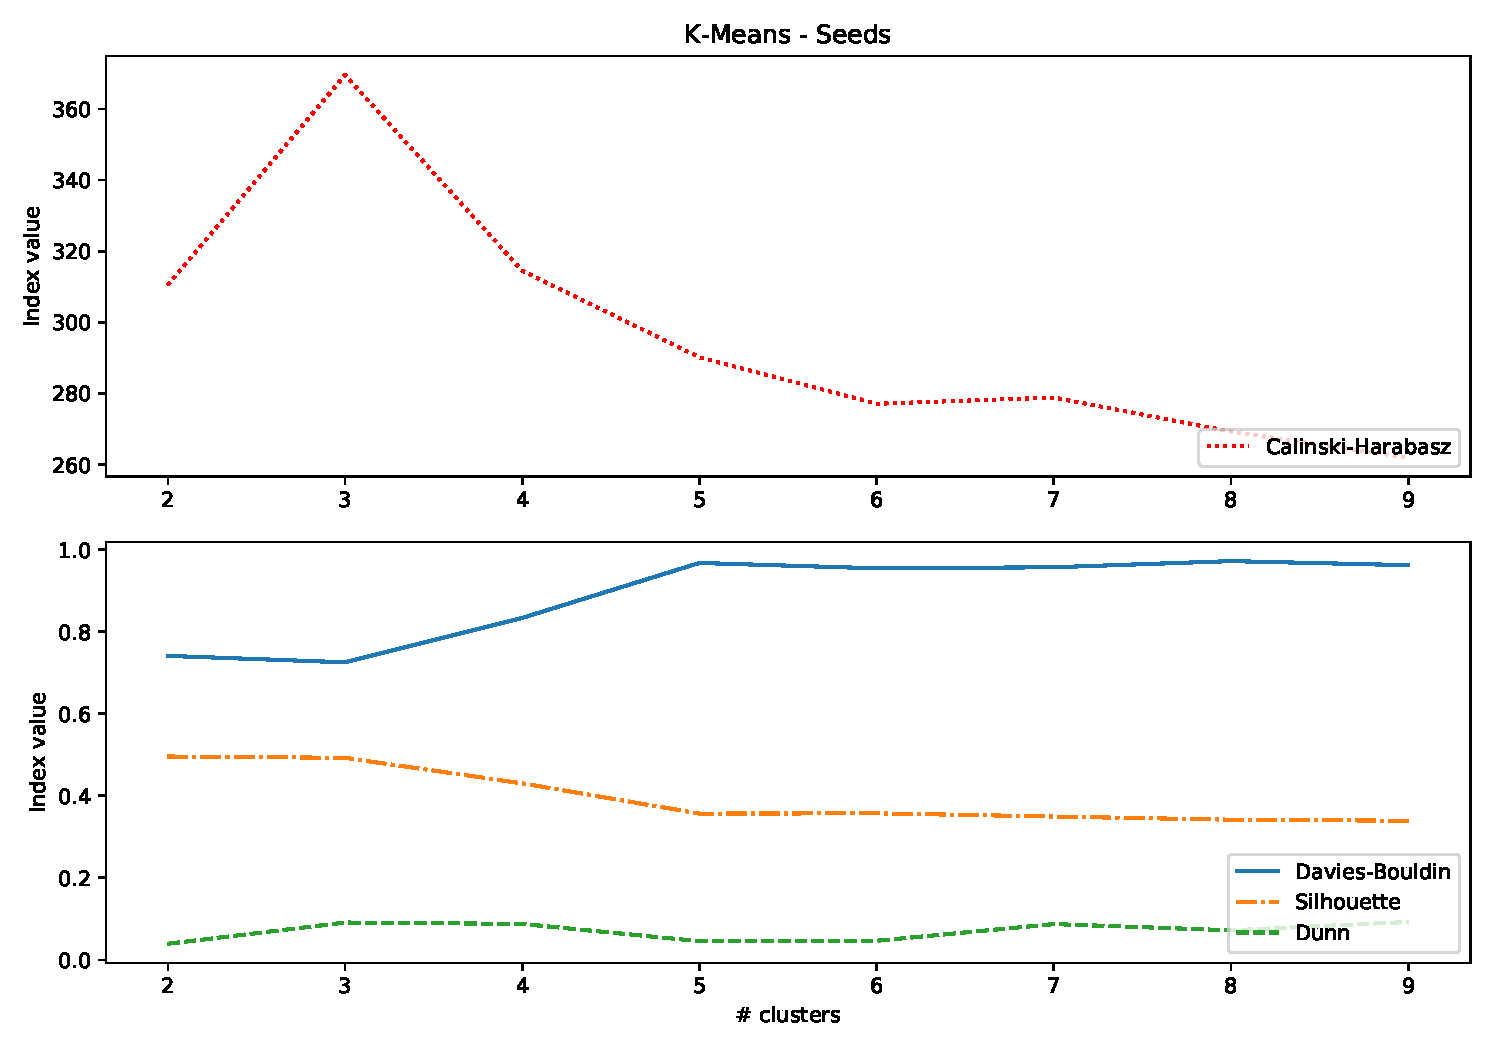
\includegraphics[width=1.0\textwidth]{images/kmeans_seeds_index_plot.pdf}
\end{center}
\label{fig:kmeans_seeds_comparison_plot}
\end{figure}

Looking at figure \ref{fig:kmeans_seeds_comparison_plot} (one line for each index, two panels because of the vastly different scale of \gls{CH}) one can see a clear maximum in \gls{CH} value and a local maximum in \gls{DI} as well as a change in slope for \gls{SI} at three clusters each. Following the described logic, \gls{DB} suggests also considering five clusters as an option. 

As mentioned in section \ref{sec:data_description} this dataset originally comes with labels which allows to use them as a benchmark to see how the clustering performs. Plotting (figure \ref{fig:kmeans_seeds_tsne}) two dimensional representations (see t-SNE in section \ref{sec:frontend_description}) of the K-Means clustered result and the original data shows a few things: the algorithm has, as expected, produced non-overlapping mostly contiguously shaped clusters in contrast to the original data. However using three clusters has generally produced a reasonably good fit, as is supported by an accuracy of 89.5\%, precision of 90\% and recall of 89.5\% to name a few standard metrics.

\begin{figure}[H]
\caption{Example with 1 dimension and 10 points bad starting position}
\begin{center}
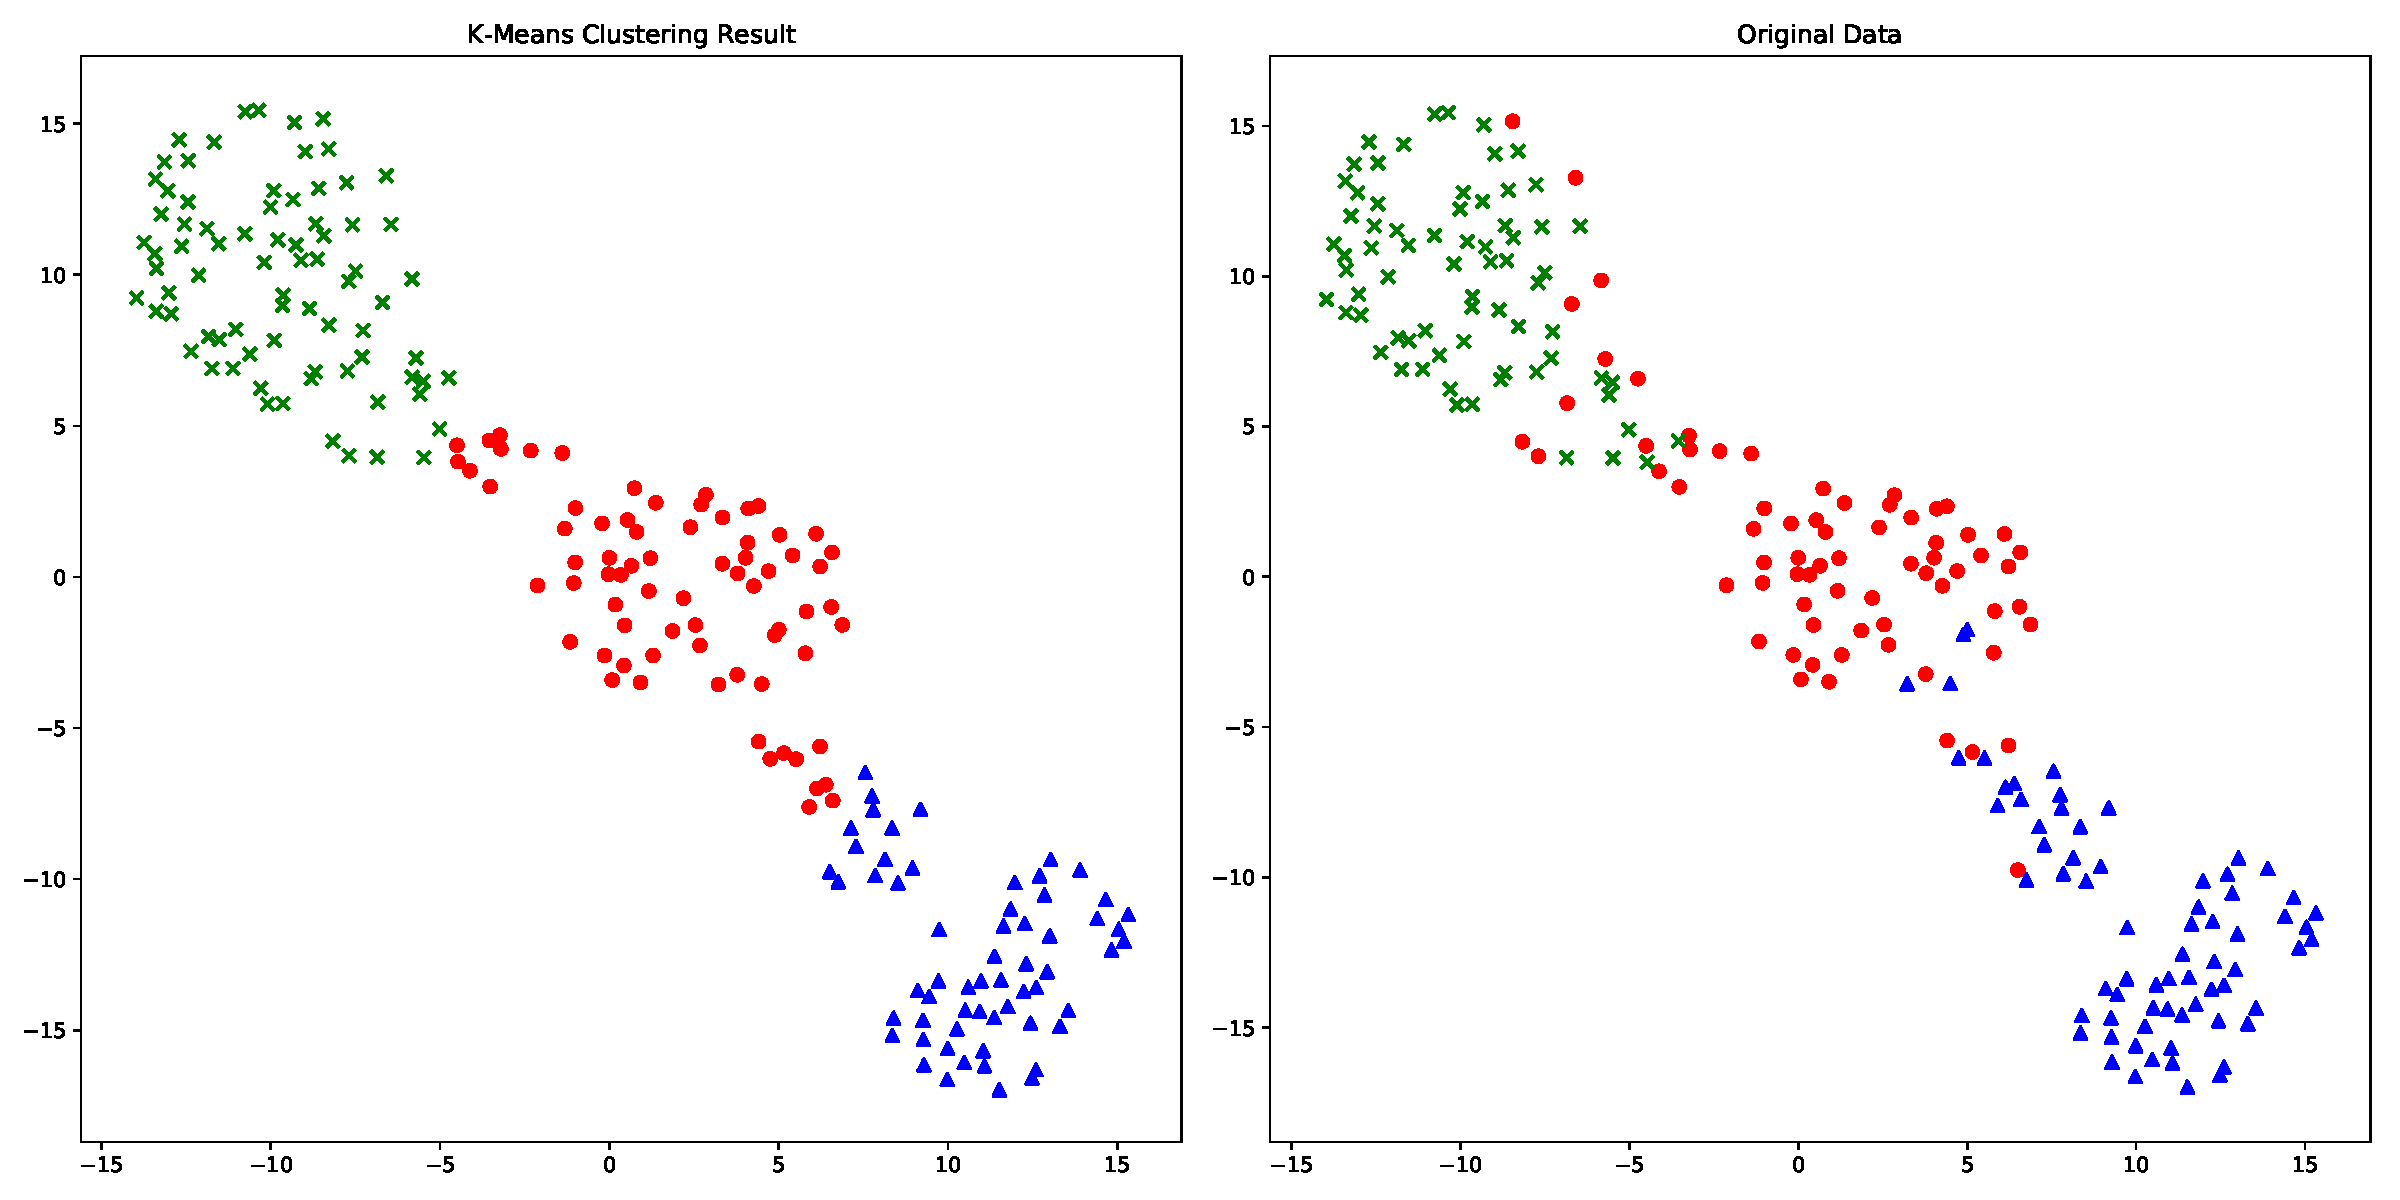
\includegraphics[width=1.0\textwidth]{images/kmeans_seeds_tsne.pdf}
\end{center}
\label{fig:kmeans_seeds_tsne}
\end{figure}

%continuous data in all features makes application straight forward
%as shown in table \ref{tab:k-means_seeds_table} data on how many clusters to choose not clear
%looking at chart in \ref{fig:kmeans_seeds_indices_plot} makes comparison easier. shows \gls{CH} with significant signal at three clusters and \gls{DI} flattening out after three clusters while \gls{SI} falling after three clusters. only \gls{DB} highest at seven clusters. in light of this analysis it doesn't seem unreasonable to select three clusters as the best fit. looking at the data in 3d, see figure

\subsubsection{Mall Customers K-Means}
\textit{written by B.L.}\\

As one of the features is categorical (gender), this is not an ideal application of the K-Means clustering method. The categories can be resolved into discrete values so that calculations can be run, but the arbitrary nature of this does not really allow for good interpretation of the results. An exemplary three dimensional plot \ref{fig:kmeans_customers_3d} shows the issue: 
\begin{wrapfigure}{r}{0.5\textwidth}
  \centering
    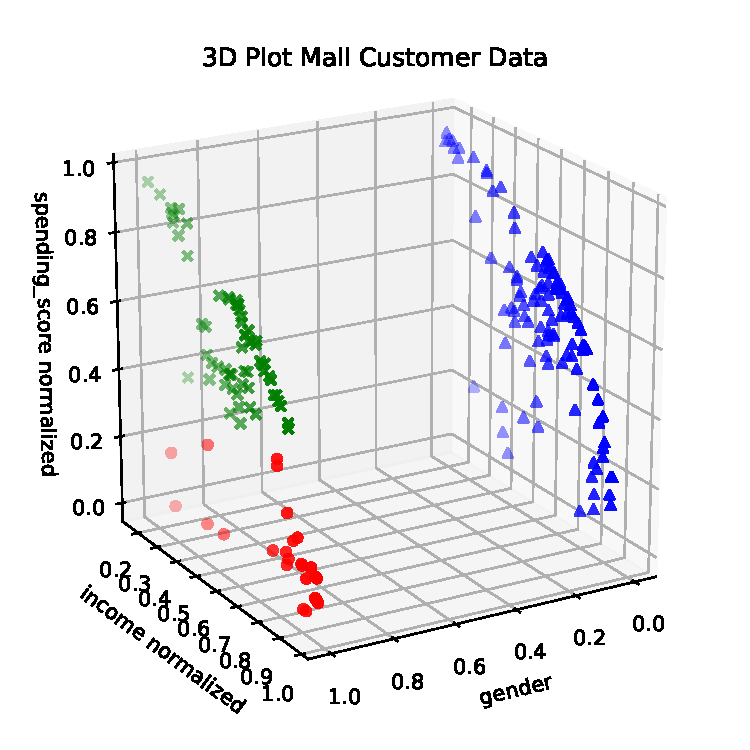
\includegraphics[width=0.48\textwidth, clip]{images/kmeans_customers_3d.pdf}
  \label{fig:kmeans_customers_3d}
  \caption{Split Data Due To Categorical Feature}
\end{wrapfigure}
gender is represented on the z-axis and the two manifestations simply rip the data into two partitions. When gender is encoded as 0 and 1, this showed almost no effect. When using 0 and 100, it leads to a doubling in the index-recommended number of clusters. One attempt to deal with this is to scale all data between 0 and 1 but this aggravated the problem instead of improving on it. Extensions of the K-Means method have been devised to deal with this type of data (as described in section \ref{subsec:method_kmeans}) but their application here seems beyond the scope of this work. Using the gender feature also does not improve scores in the evaluation methods used. Given these circumstances, considering plot \ref{fig:kmeans_customers_indices_plot} suggests considering the results for 2, 3 or 8 clusters.

\begin{figure}[h]
\caption{K-Means Mall Customers Dataset Indices by Number of Clusters}
\begin{center}
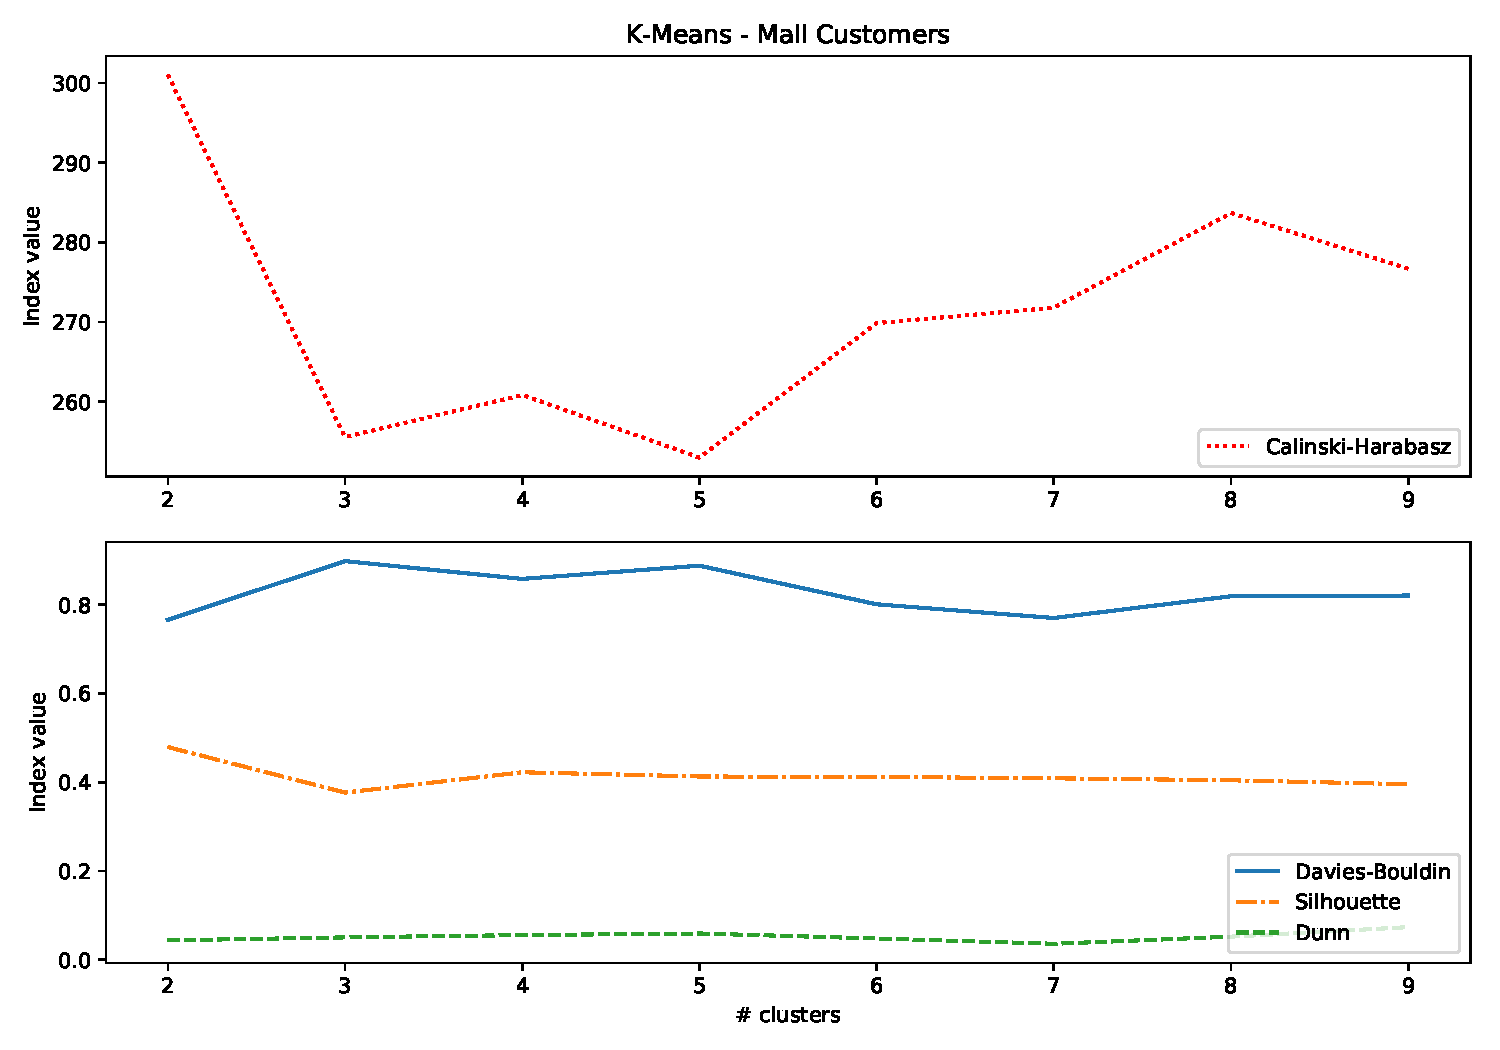
\includegraphics[width=1.0\textwidth]{images/kmeans_customers_index_plot.pdf}
\end{center}
\label{fig:kmeans_customers_comparison_plot}
\end{figure}

The dataset contains four features, three of which have a measurable and interpretable impact on clustering, which lends itself to a visual comparison in three dimensional space. Figure \ref{fig:kmeans_customers_3d_multi} shows three plots, one for each suggested number of clusters. The highest overall evaluation scores were achieved for two clusters and purely from a visual standpoint this seems to hold up.

\begin{figure}[h]
\caption{Example with 1 dimension and 10 points bad starting position}
\begin{center}
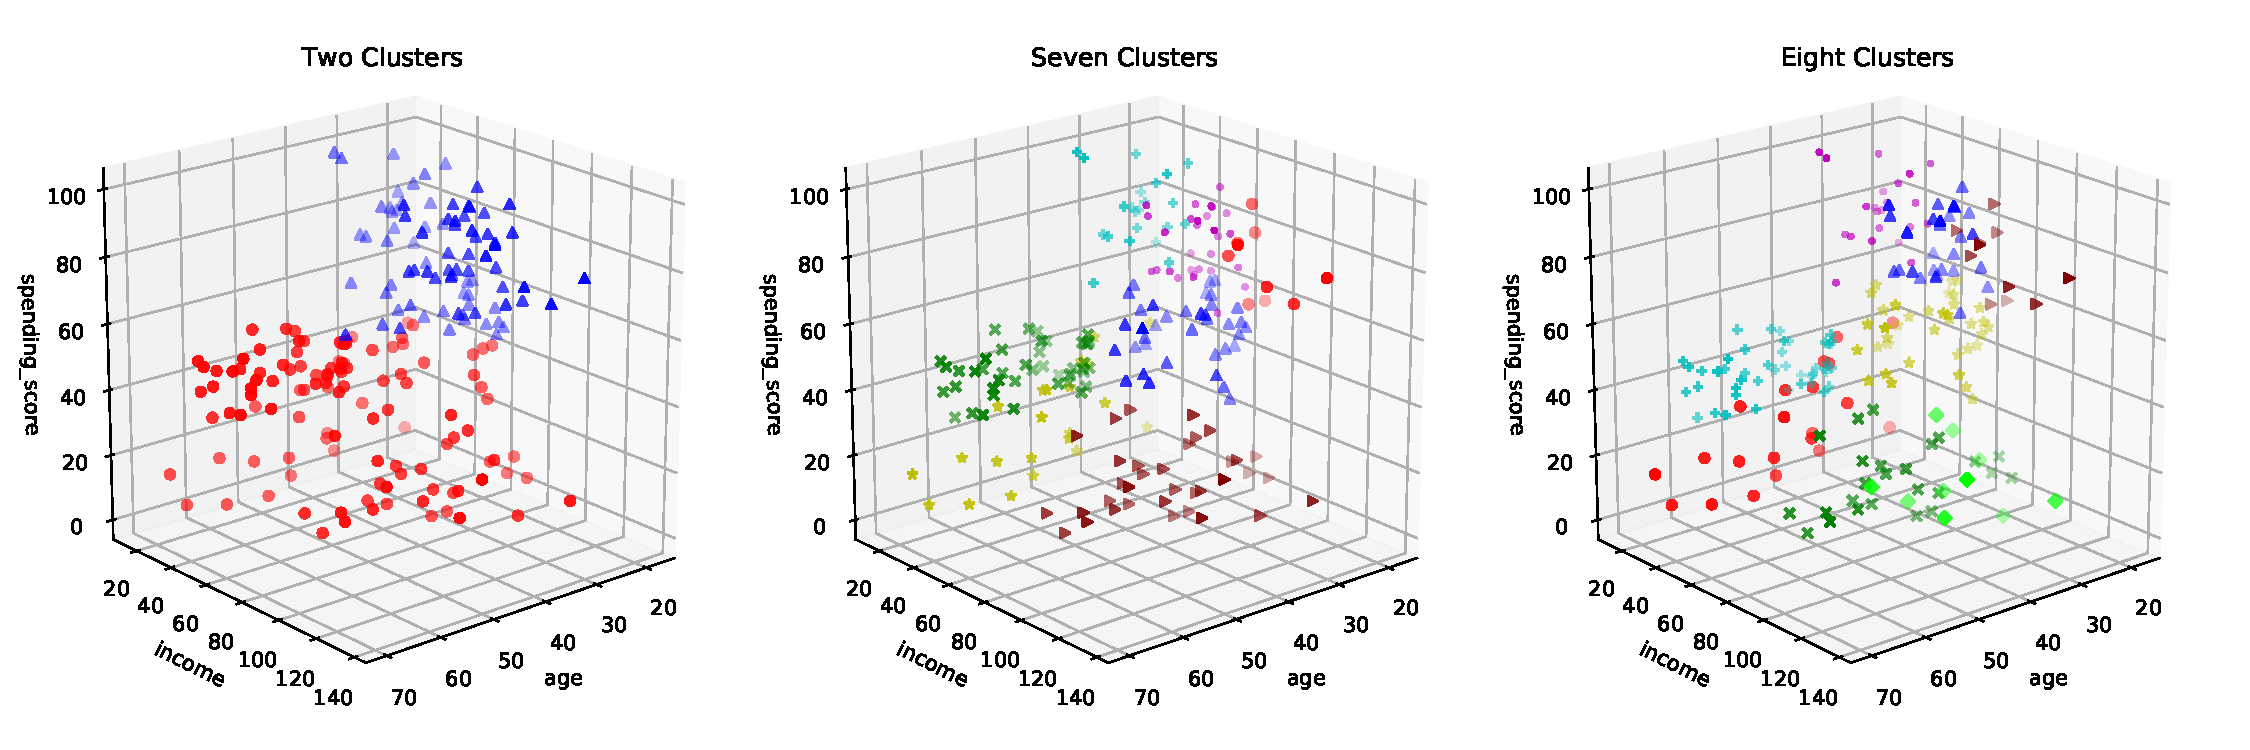
\includegraphics[width=1.0\textwidth]{images/kmeans_mall_3d_multi.pdf}
\end{center}
\label{fig:kmeans_customers_3d_multi}
\end{figure}

%Rotating the plot shows that both partitions contain very similar clusters but due to the way K-Means works they are not recognized as the same. The data shows either two clusters (simply male cluster and female cluster) or an ideal number of clusters double the amount perceived by a human to be reasonable.

\subsubsection{Housing K-Means}
\textit{written by B.L.}\\

This dataset is challenging for K-Means clustering due to the high number of features. As described in section \ref{subsec:method_kmeans} the concept of distance does not hold up well in high dimensional cases. Attempts to transform the data into lower dimensional representations through principle component analysis did not yield an improvement in clustering performance. Data in figure \ref{fig:kmeans_housing_indices_plot} suggests to consider 2, 3, 4 or on the other hand a very high number of clusters.

\begin{figure}[h]
\caption{K-Means Housing Dataset Indices by Number of Clusters}
\begin{center}
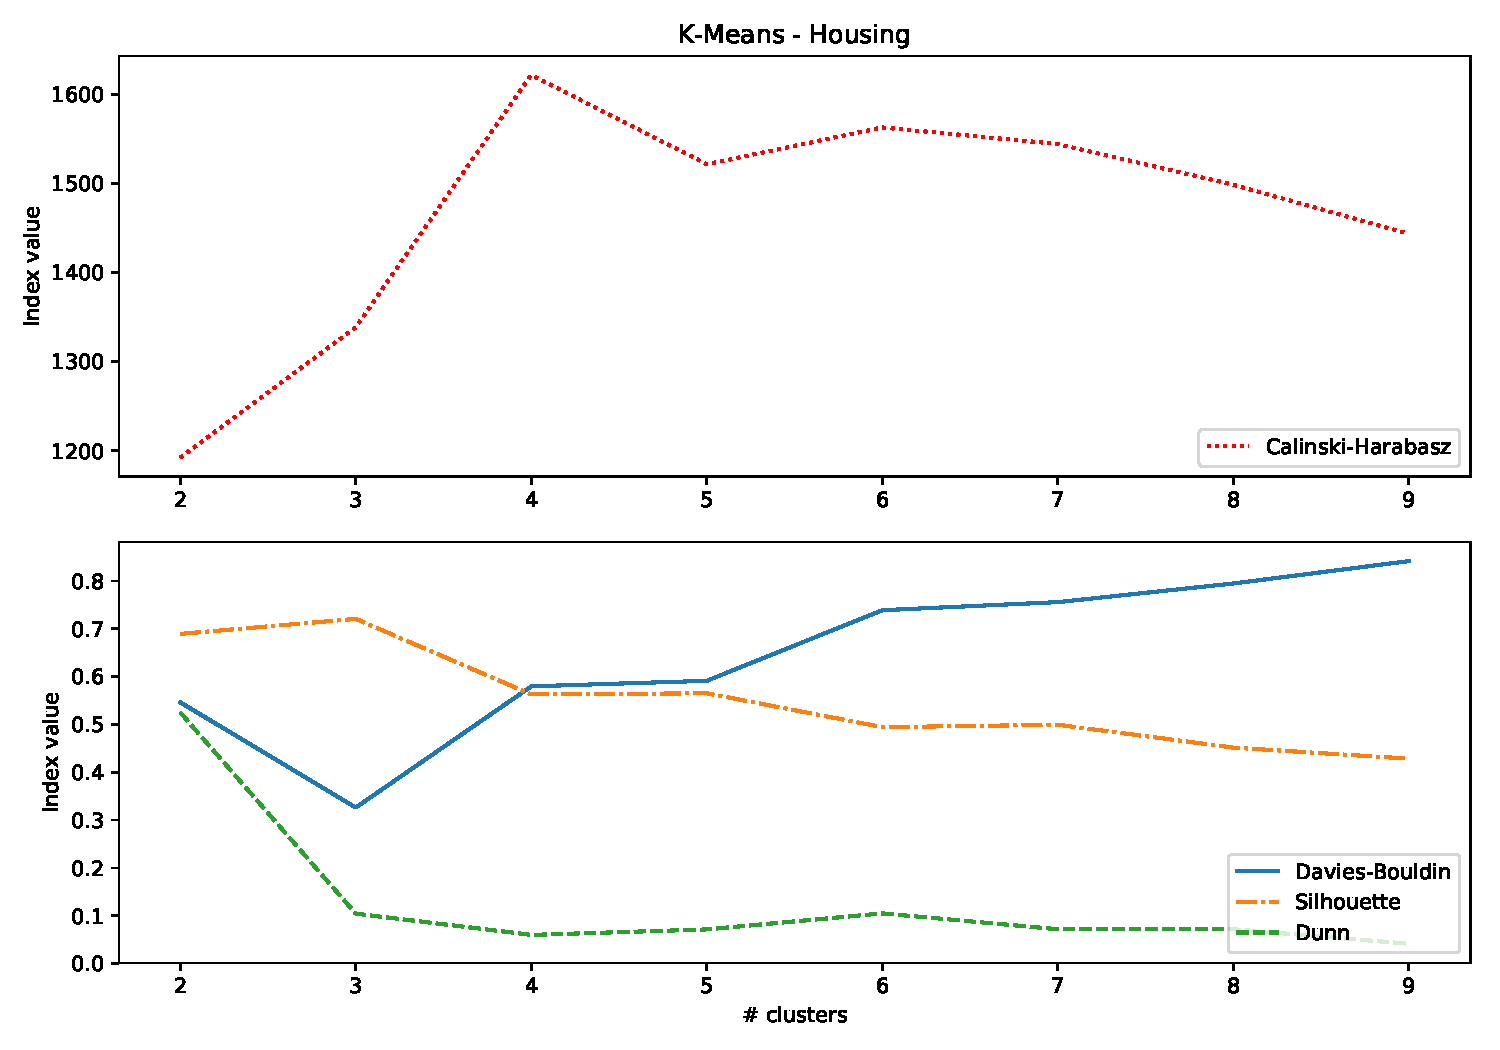
\includegraphics[width=1.0\textwidth]{images/kmeans_housing_index_plot.pdf}
\end{center}
\label{fig:kmeans_housing_comparison_plot}
\end{figure}

Due to the high dimensionality of the data, looking at different angles in three dimensions to get an understanding is not feasible. Therefore a two dimensional transformation (t-SNE, see section \ref{sec:frontend_description} will help. Figure \ref{fig:kmeans_housing_2d_comparison} shows the case of two, three and 15 as representation for a significantly higher number of clusters. From a visual standpoint, two and three clusters seem to capture the visibly separated parts of the data quite well, while the high cluster count suggests it might be reasonable to consider the idea of there being a much more complex underlying structure to the data which is not well captured through the method at hand.

\subsubsection{Wine K-Means}
\textit{written by B.L.}\\

The wine dataset again presents a challenge due to its high feature count, the highest of all the datasets in this comparison as well as having one discrete feature. Dimensionality reduction helps to speed up calculation but does not show an improvement in evaluation index performance. The plot of evaluation indices in figure \ref{fig:kmeans_wine_indices_comparison} gives an indication around eight to ten clusters

\begin{figure}[h]
\caption{K-Means Wine Dataset Indices by Number of Clusters}
\begin{center}
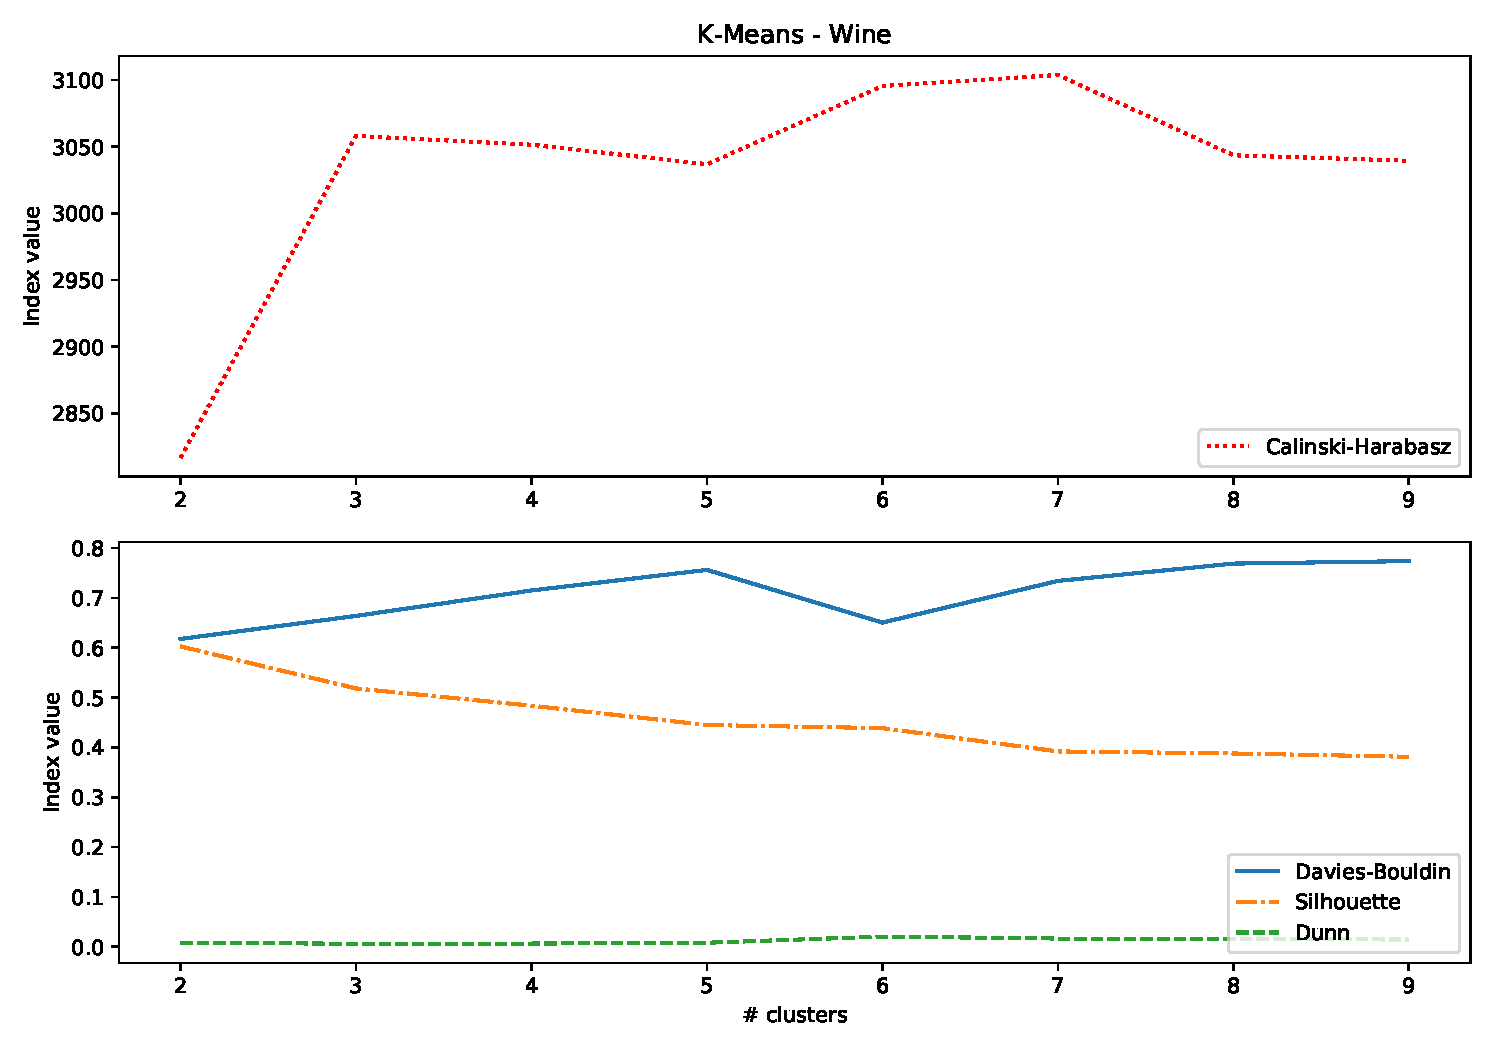
\includegraphics[width=1.0\textwidth]{images/kmeans_wine_index_plot.pdf}
\end{center}
\label{fig:kmeans_wine_indices_comparison}
\end{figure}

but looking at the two dimensional transformed data in figure \ref{fig:kmeans_wine_tsne} does not allow for any visual evaluation concerning the quality of fit. The result is inconclusive and without a focus on feature engineering other methods may be better suited to deal with this dataset.

\begin{figure}[h]
\caption{K-Means Wine Dataset Indices by Number of Clusters}
\begin{center}
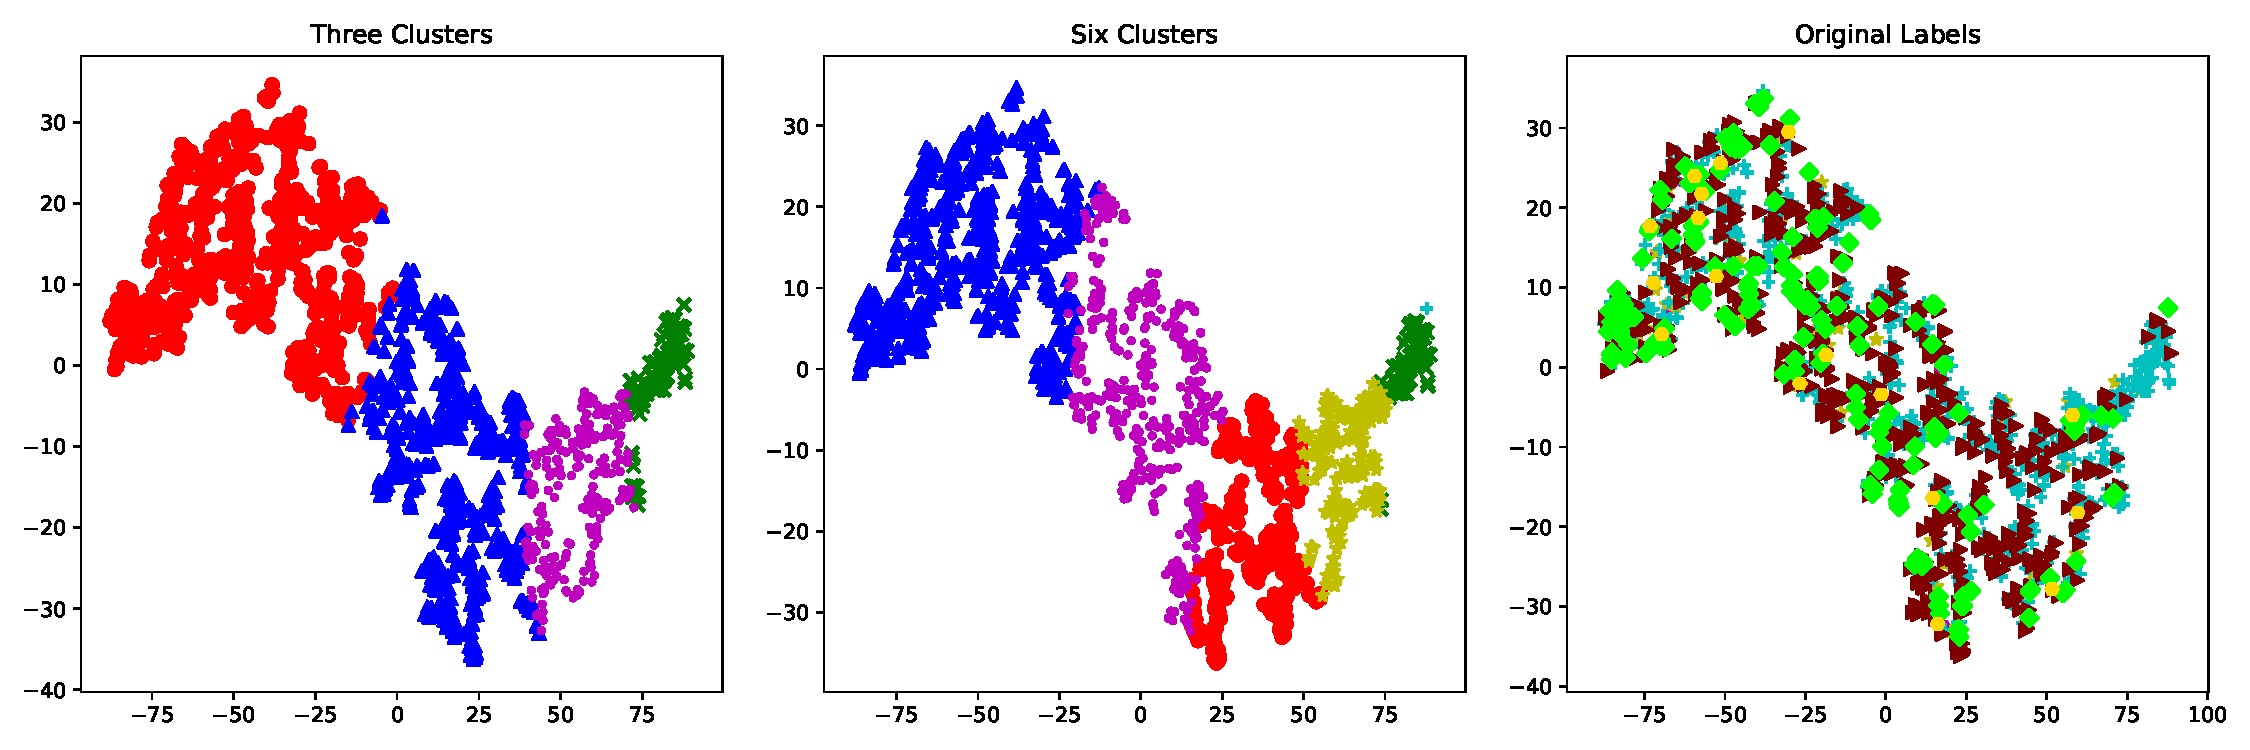
\includegraphics[width=1.0\textwidth]{images/kmeans_wine_tsne.pdf}
\end{center}
\label{fig:kmeans_wine_tsne}
\end{figure}


% \begin{itemize}
% \item What are the results and how are they measured?
% \end{itemize}